\documentclass[12pt]{article}

\usepackage{booktabs}
\usepackage{dcolumn} 
\usepackage{epstopdf}
\usepackage{fourier}
\usepackage{fullpage}
\usepackage{graphicx}
\usepackage{hyperref}
\usepackage{longtable} 
\usepackage{natbib}
\usepackage{rotating}
\usepackage{tabularx}
\usepackage{amsmath}
\usepackage{threeparttable} 
\usepackage{setspace} 
% \usepackage{algorithmic} 
% \usepackage{algorithm2e}

\hypersetup{
  colorlinks = TRUE,
  citecolor=blue,
  linkcolor=red,
  urlcolor=black
}

\newcommand{\qu}[1]{``#1''}
\newcommand{\starlanguage}{Significance indicators: $p \le 0.05:*$,
  .$p \le 0.01:**$ and $p \le .001:***$.} 


\newcommand{\numRaters}{127}
\newcommand{\numOccupations}{99}
 

\begin{document} 

\title{Perceptions of Occupations: \\ Good on Wages, Bad on Changes}

\date{\today}

\author{John J. Horton \\ Leonard N. Stern School of Business \\ New
  York University\footnote{Author contact information, datasets and
    code are currently or will be available at
    \href{http://www.john-joseph-horton.com/}{http://www.john-joseph-horton.com/}. 
    Thanks to Alex Gedranovich for excellent research assistance. 
} \and Adam Kapelner \\ Department of Mathematics \\ Queens College, CUNY}
\maketitle

\begin{abstract}
\noindent  
A sample of labor market participants were asked to estimate the wage and projected employment growth for a selection of occupations;
they also reported how many people they knew working in that occupation, which was used to create a ``social knowledge'' index. 
Collectively, respondents have good knowledge about wages --- their wage estimates can explain more than 50\% of the variation in actual log wages as reported by the United States Bureau of Labor Statistics.
However, it appears they know very little about the direction of projected employment trends; their predictions about future employment are no better than chance. 
Despite poor overall predictions about employment trends, individual predictions were substantially improved if the respondent had better social knowledge about that occupation.
\newline 
\newline 
\noindent JEL J01, J24, J3
\end{abstract} 

% \doublespacing

\section{Introduction}
When planning a career, a labor market participant should know both what a career can pay and the future prospects of that career.
Misinformation about the current and future prospects of different occupations could lead to poorly considered career and human capital allocation decisions. 
This paper attempts to asses the quality of labor market knowledge. To do so, we employ
a convenience sample of the US population drawn from Amazon Mechanical Turk (MTurk). For the top 100 most common American careers, we compare respondent per-occupation estimates of wages and respondent employment growth estimates to gold-standard estimates provided by the Bureau of Labor Statistics (BLS). 
The paper also attempts to understand how predictive accuracy is affected by ``social knowledge'' of that occupation, where social knowledge is an index based on how many people the respondent knows working in that occupation.

Collectively, the ``wisdom of crowds'' hypothesis seems to hold regarding wages: 
excluding some notable exceptions, the mean of estimates of wages were quite accurate. 
However, respondents did underestimate the wages of higher wage jobs, though it is unclear how much of this is due to the selected nature of respondents. 
%Is lackluster knowledge of high income wages due to some cognitive bias that you know of? Also, I'm not sure what you mean by "selected nature of respondents"

However, the same wisdom of the crowds does not apply when estimating future career projections.
Respondents were asked whether the fraction of people employed in an occupation will go up, go down or stay the same. 
Collectively, they do not predict better than chance when their answers are compared to the BLS projections. 
However, the more social knowledge a respondent has about an occupation, the better their prediction on the employment trend for that occupation. %How much better? (we should probably but a sentence here)

The improvement in predictive accuracy from social knowledge is found despite our controlling for both the respondent and the occupation.
This analysis rules out the possibility that some occupations are easier to predict and many people know workers in those occupations; 
they also rule out the possibility that people with more social connections are better predictors.
While still not causal, the non-causal channels for why social knowledge seems to improve predictive accuracy is far smaller than if we had only cross-sectional data. %What does "channels" mean?

%also - did you elicit demographics? Age is a good thing to control for. Young people may know less than older people.

The ability to include both kinds of controls illustrates an offsetting advantage to using MTurk: 
while still a convenience sample, MTurk provides a way to obtain a large number of responses even for a questionnaire that a ``representative'' sample would find tedious and be unlikely to complete carefully.
This feature of MTurk is increasingly being used for questions in economics  \citep{kuziemko2013elastic, saez2013generalized}. 

There is also evidence that suggests MTurk convenience samples are better than in-person convenience samples (a common sample published in social science) and can be similar to true probability samples. \citet{Berinsky2012} found MTurk respondents are similar in demographic profile to the gold-standard probability sample except they are younger, more politically liberal and pay more attention to cognitive tasks. We believe that the sample being younger biases our results downwards as younger poeple should be less likely to predict both wages and future trends due to inexperience. We do not believe political orientation of need for cognition will have an effect on the generalizability of the associations this study reveals.

There are conceptually similar papers to this one, but most of have focused on schooling decisions.  
For example, \cite{dominitz1996} elicited the returns to schooling from a convenience sample of high school students and undergraduates. 
Another example is \cite{jensen2010perceived}, which also focuses on returns to schooling, but includes an experimental information intervention that increased later schooling.   %What is an "information intervention"? Maybe this deserves a few more words
General questions about the labor market --- including some questions about various occupations --- were part of the National Longitudinal Survey (NLSY) for a brief period in the Knowledge of the World of Work (KWW) subtest \citep{kohen1975}, though the nature of the questions was quite dissimilar to the questions asked in this paper. 
This is the first paper we are aware of that focuses explicitly on occupational knowledge.

There are many potential sources of knowledge about careers: career counselors, formal government statistics and informal channels like family and friends. 
There is a long-standing interest in how informal channels in labor markets affect outcomes \citep{rees1966information, stigler1962information}, but the very informality of these channels has made them difficult to study. 
Interest in these informal channels --- particularly referrals --- is going through a renaissance as it becomes easier to run experiments \citep{pallais2013referential} and obtain high-quality administrative data \citep{burks2013value}.   
This paper focuses on a social ``stage'' manifesting earlier than referrals by assessing how social connections mediate the knowledge needed to decide which opportunities to pursue.  
If the patterns discovered here generalize, gaps in our knowledge might be readily fixed: 
several studies have highlighted the powerful effects from purely informational interventions (e.g., \citealp{dupas2009teenagers, card2010inequality}).
If first-hand social knowledge is an important disseminator of labor market information, this suggests that more isolated individuals are exposed to a narrow slice of occupational possibilities putting them at a labor market disadvantage, thereby contributing to inequality. 

% \cite{hlavac2013} for stargazer. 
% \cite{ward1992} 
% \cite{betts1996students} 
% \cite{webbink2004} 
% \cite{dominitz1996} 

\section{Data collection and description} 

For the top 100 US occupations by employment totals as measured by the May 2013 Occupational Employment Statistics (OES),\footnote{\url{http://www.bls.gov/oes/}}  respondents from Amazon Mechanical Turk were asked
(1) whether they knew what the occupation consisted of 
(2) how many people they knew who held the occupation, if any,  
(3) their estimate of the hourly wage for the occupation
and (4) whether in the future employment in the occupation would rise, fall or stay the same.
The actual survey interface presented to respondents is shown in Figure~\ref{fig:survey} in Appendix~\ref{sec:survey}. 
There were no incentives for correct answers and the short time most workers spent on any tasks suggests they were not performing research. 

A total of \numRaters\, respondents participated in the survey. 
Each occupation was evaluated by 30 different respondents, though for our analysis we only included occupations where at least 20 out of the 30 respondents knew what the occupation was.
We then further restricted the sample to only observations where the respondent knew what that occupation was. %I'm not sure what's going on here. I tihnk we only need to talk about one of the restrictions.
Appendix~\ref{sec:additional} contains descriptive statistics of respondent knowledge about all occupations originally included in the survey.   

For ``ground truth'' on occupational wages, we simply used the estimated hourly mean wage from the OES.
However, for occupations where hourly wages are not available, we computed an estimated hourly wage based on a 40 hour week for 50 weeks a year.  
For employment predictions, we computed the percentage change from the 2010 employment level (the fraction of the workforce in each occupation) to the the 2020 employment projections. 
I classified changes that were $\pm$ 5\% as ``Stay the Same'' (getting a value of $0$) and those greater than 5\% getting a value of $1$ and those with a greater than 5\% decrease getting a value of $-1$.  
The actual language of my survey question was ``20 years'' in the future. 
While this is not the period over which we have official BLS predictions, we worried that with too short of a time period many respondents would choose ``Stay the same'' and hence the request for a 20 year prediction. %I don't understand: why didn't you ask for a "10yr" prediction? I think this needs another sentence of justification.

For the social knowledge measure, respondents were asked how many individuals they knew in an occupation. 
The choices were $0$, $1$, $3-10$ and \qu{more than $10$.} 
To construct a social index, these bins were coded as ``0'', ``1'', ``2'' and ``3'', respectively and then normalized with respect to the population of all responses across occupations.

%I'm not sure we explained enough here. In the next section we talk about fixed effects for each respondent. What was the breakdown of number of questions answered by each respondent? 

\section{Results}

\subsection{Predictions about wages and employment growth}

To compare respondent predictions to BLS estimates, we regressed the BLS estimate on the associated respondent estimate. 
In Column~(1) of Table~\ref{tab:predictions}, the outcome variable is the log of the actual mean wage for the occupation. 
The regressor is the log of the respondent's wage estimate for that occupation. 
The regression includes a respondent-specific fixed-effect and standard errors are clustered at the level of the respondent. 
%not that it's going to matter, but here's a situation where random effect models can pay the rent. You can reasonable assume that a respondent's mean wage / prediction is drawn from a normal distribution. Thus, you don't have to blow 127 degrees of freedom on fixed effects. You'll get a bunch more power too
We can see that the estimated wage is not only highly significant and positive, but the $R^2$ for the model is quite high, with these estimates collectively explaining more than half the variation, even after the degrees of freedom correction. 


% Table created by stargazer v.5.1 by Marek Hlavac, Harvard University. E-mail: hlavac at fas.harvard.edu
% Date and time: Mon, Mar 02, 2015 - 03:31:22 PM
\begin{table}[!htbp] \centering 
  \caption{Predictions about wages and employment trends} 
  \label{tab:predictions} 
\small 
\begin{tabular}{@{\extracolsep{5pt}}lcc} 
\\[-1.8ex]\hline 
\hline \\[-1.8ex] 
 & \multicolumn{2}{c}{\textit{Dependent variable:}} \\ 
\cline{2-3} 
 & Log Mean Occupational wage & Pred. Employment change \\ 
\\[-1.8ex] & (1) & (2)\\ 
\hline \\[-1.8ex] 
 Estimated log wage & 0.765$^{***}$ &  \\ 
  & (0.023) &  \\ 
  & & \\ 
 Estimated employment change &  & $-$0.030$^{*}$ \\ 
  &  & (0.013) \\ 
  & & \\ 
\hline \\[-1.8ex] 
Respondent FE & Yes & Yes \\ 
Observations & 1,898 & 1,898 \\ 
R$^{2}$ & 0.569 & 0.059 \\ 
Adjusted R$^{2}$ & 0.540 & $-$0.004 \\ 
\hline 
\hline \\[-1.8ex] 
\end{tabular}
\\
\begin{minipage}{0.95 \textwidth}
{\footnotesize \emph{Notes:}
           The sample for both regressions reported in this table are all the repsponses where the respondent said they knew what an occupation consisted of.
In Column~(1), the dependent variable is the actual log mean wage for that occupation (from the May 2013 OES estimates from the BLS), while in Column~(2) the dependent variable is an index for whether the BLS predicts that by 2020 the fraction employed in that occupation will grow by more than 5\% (outcome = 1), fall by more than 5\% (outcome = -1) or will not change by more than 5\%, positive or negative (outcome = 0).
The important independent variable in both regressions is the respondent's prediction.
Both regressions include a respondent-specific standard error. 
Standard errors are clustered at the level of the individual respondent. 
\starlanguage }
\end{minipage}
\end{table}
 %Why is the intercept not shown here? It should be close to zero.

The regression approach masks a pattern in responses that is readily visible when actual wages are plotted against mean worker estimates. 
Figure~\ref{fig:prediction_scatter} is a scatter plot of the log actual wages (y-axis) versus the mean of log predicted wages (x-axis) for each occupation. 
Deviations from the 45 degree line indicate prediction errors. 
There are two notable features of the data clearly illustrated by the the plot. 
We can see that respondents systematically underestimate the wages of occupations at the high end of the distribution.\footnote{The only occupation that workers substantially over-estimate is the home health aide category --- perhaps because of a mistaken belief that this is the nursing occupation.}  
Some outliers --- both positive and negative --- are labeled with the occupation title.  
Many of the extreme outliers are under-estimates of the wages of managerial occupations. 

\begin{figure}
\caption{Perceived hourly wages versus actual hourly wages \label{fig:prediction_scatter}} 
\centering 
\begin{minipage}{0.90 \linewidth}
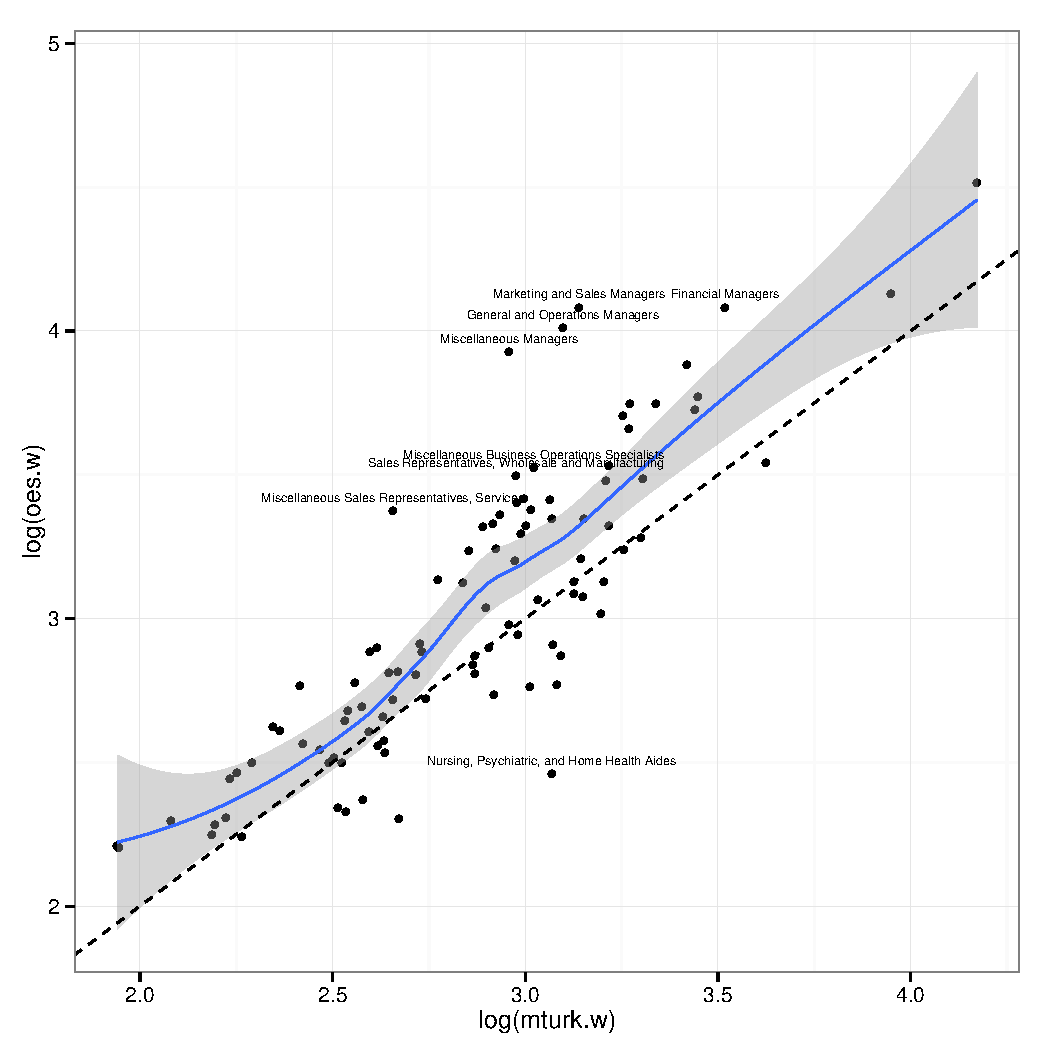
\includegraphics[width = \linewidth]{./plots/predicted_v_actual.pdf} 
\\
\emph{Notes:} This plot shows the actual log mean wage versus the mean log wages versus predicted wages.  
\end{minipage}  
\end{figure} 
%I'm wondering if it's worth adding a grey line to each of the points in the plot to indicate confidence interval.

In Column~(2), Table~\ref{tab:predictions}, the outcome variable is the expected change in employment on the ``Go Down'' = -1, ``Stay the same'' = 0, ``Go up'' = 1 scale and the independent variable is the respondent's prediction. 
As with the wage predictions, a respondent-specific fixed effect is included and standard errors are clustered at the respondent level. 
To the extent that the regression has any predictive power, it is gained by \emph{negatively} weighting predictions:
in sharp contrast to the wage prediction results, there is essentially no relationship between BLS projections and individual projections. 

%Did you test the interaction? That is, if the worker did well on predicting wage, was their prediction of projection more likely correct? You can do that by running the regression

%BLS growth projection (-1/0/1) = intercept + fixed respondent effect + respondent growth projection prediction + squared_error(respondent wage prediction, BLS gold standard wage) + beta * respondent growth projection prediction * squared_error(respondent wage prediction, BLS gold standard wage) + noise clustered at the respondent 

%if beta does not turn out to be significant, our argument is stronger "further, there's no correlation between knowing the wage and the projection." If it's significant, it will be weak; it can't be strong because column 2 shows an Rsqd ~ 0. So there, it still works for your argument.

\subsection{Social knowledge and predictive accuracy}

I now consider whether social knowledge of an occupation improves individual predictive accuracy. 
In Table~\ref{tab:fe_errors}, Column~(1), the dependent variable is the respondent's prediction error in wages, defined as the absolute value in the difference in log wages between the respondent's estimate and the BLS value.  
In Table~\ref{tab:fe_errors}, Column~(2), the dependent variable is the respondent's prediction error in employment trends, similarly defined as the absolute value in the difference in projects. 
For both regressions, both occupation- and respondent fixed-effects are included and standard errors are clustered at the respondent level.  


% Table created by stargazer v.5.1 by Marek Hlavac, Harvard University. E-mail: hlavac at fas.harvard.edu
% Date and time: Mon, Mar 02, 2015 - 03:31:23 PM
\begin{table}[!htbp] \centering 
  \caption{Social and errors in occupational wage and employment trajectories} 
  \label{tab:fe_errors} 
\begin{tabular}{@{\extracolsep{5pt}}lcc} 
\\[-1.8ex]\hline 
\hline \\[-1.8ex] 
 & \multicolumn{2}{c}{\textit{Dependent variable:}} \\ 
\cline{2-3} 
 & Wage Error & Employment Trend Error \\ 
\\[-1.8ex] & (1) & (2)\\ 
\hline \\[-1.8ex] 
 Social Knowledge Index & $-$0.030 & $-$0.054$^{**}$ \\ 
  & (0.025) & (0.019) \\ 
  & & \\ 
\hline \\[-1.8ex] 
Respondent FE & Yes & Yes \\ 
Occupation FE & Yes & Yes \\ 
Observations & 1,898 & 1,898 \\ 
R$^{2}$ & 0.373 & 0.327 \\ 
Adjusted R$^{2}$ & 0.304 & 0.252 \\ 
\hline 
\hline \\[-1.8ex] 
\end{tabular}
\\
\begin{minipage}{0.95 \textwidth}
{\footnotesize \emph{Notes:} This table reports the effects of social and general knowledge on a
respondent's prediction error, while controlling for worker and
occupation specfic effects. In Columns (1) the dependent
variable is MSE in wage prediction, while in Column (2), the
dependent variable is an indicator for incorrectly predicting the
direction of employment growth in that occupation. \starlanguage }
\end{minipage}
\end{table}


For wages, in Column~(1), we can see that social knowledge is associated with reduced error, but the effect size is small and not significant. 
For project employment in Column~(2), however, we can see that greater social knowledge is strongly associated with lower error in projected employment.  

\section{Discussion}

One possible explanation for error in prediction for high-wage occupations is that occupations at the high end are more likely to be salaried, which may weaken workers' ability to infer hourly wages. 
Also, workers on Amazon Mechanical Turk tend to have lower than average wages and tend to be younger than the population at large \citep{ipeirotis2010demographics}. 
It is an open question whether this finding would generalize to the larger population. 

The lack of predictive ability about employment trends is perhaps, ex post, unsurprising. 
Knowing employment trends for an occupation would require a fairly sophisticated understanding of long-term trends, such as the shift away from manufacturing and towards a service-based economy and the erosion of ``middle skill jobs'' \citep{autor1998computing}.  
In contrast, learning the wages for an occupation is fairly straightforward. 

What is surprising is that employment accuracy is apparently improved through social knowledge. 
In terms of mechanisms, for the social knowledge effects, it seems likely that knowing someone who works in an occupation would grant access to more nuanced views of an occupation:
someone working in a particular field, especially one with some tenure, could probably explain how it was changing in terms of the accomplishment of the main work task, what new technologies were being used, where new sources of supply and demand were coming from and so on.  

\section{Conclusion} 

The main result of the paper is that respondents seem to have good knowledge about wages, at least collectively, but that their knowledge of projected employment---at least as predicted by the BLS---is very poor.
However, social knowledge of an occupation, i.e., knowing someone with that occupation, tends to reduce predictive error about employment trends in that occupation, even when controlling for both the respondent and the occupation. 
By controlling for both the individual and the occuopation, we can plausibly isolate the effect of social knowledge. 
It is not the case---as it would be in cross-sections---that individuals with lots of social knowledge have reduced error rates or that occupations that are well-known socially also have little error. 
While social knowledge is of course not as good as randomly assigned, reverse causation seems implausible: 
a reverse causation explanation would mean that accurate beliefs about a particular occupation causes one to have friends with someone in that occupation. 
As such, an intervention might be to expose young labor market entrants or near entrants to a wider cross section of individuals in occupations.
 
\bibliographystyle{aer}
\bibliography{kwow}

\newpage 

\appendix 

\section{Survey Materials} \label{sec:survey}  
Figure~\ref{fig:survey} shows the actual survey interface.  
Wages in the drop-down box were listed in dollar increments from \$7 to \$10, two dollar increments from \$10 to \$20, four dollar increments from \$24 to \$36 and then six dollar increments to \$70/hour.  

%Note there's a typo in "Quuestions" in this figure. You may want to correct before submission.
\begin{figure}
\centering
\caption{Survey questions \label{fig:survey}}
\begin{minipage}{0.75 \linewidth}
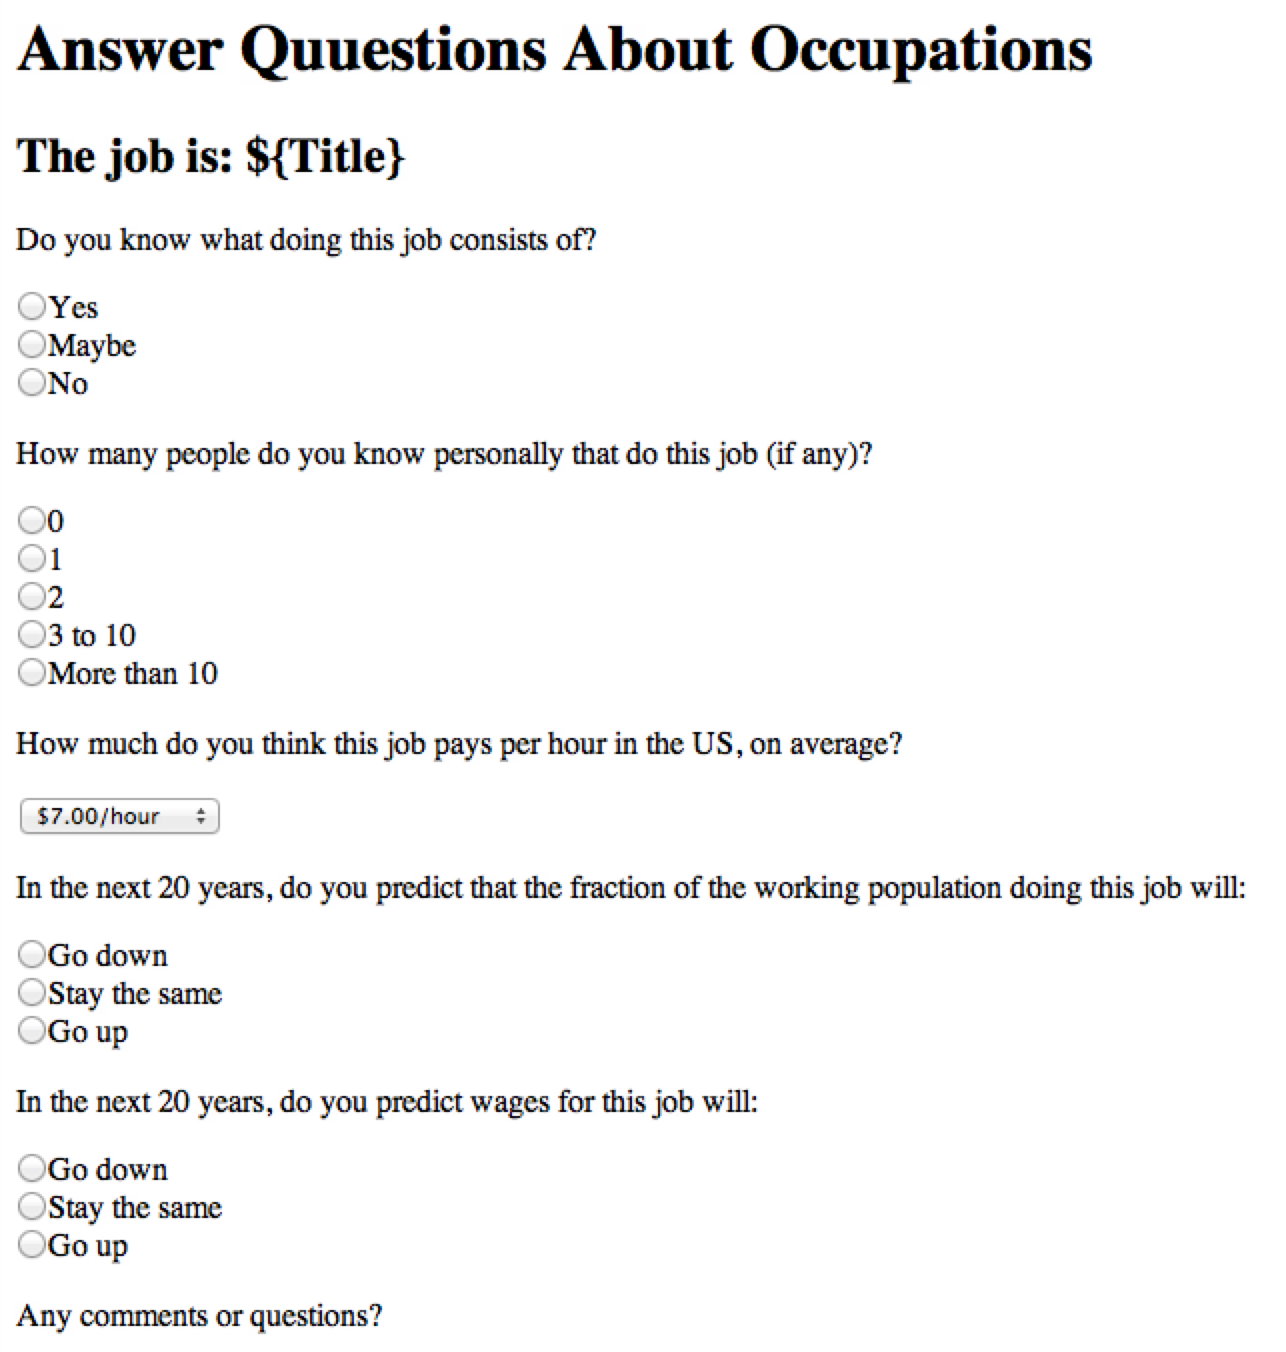
\includegraphics[width = \linewidth]{./images/survey.png}
\end{minipage}  
\end{figure} 

\section{Additional data on occupational knowledge} \label{sec:additional}

Figure~\ref{fig:by_occupation_boxplots} we plot the distribution of individual respondent log wage estimates for each occupation as a box plot. 
The actual mean and median wage for each occupation are shown as squares and triangles, respectively. 
Occupations are ordered by mean wage, from highest to lowest. 
By comparing the median of the box plot to the actual median, we can see the tendency of respondents to systematically underestimate the wages at the high end of the distribution. 

\begin{figure}
\caption{Distributions of respondent hourly wage perceptions by occupation \label{fig:by_occupation_boxplots}} 
\centering 
\begin{minipage}{0.90\linewidth}
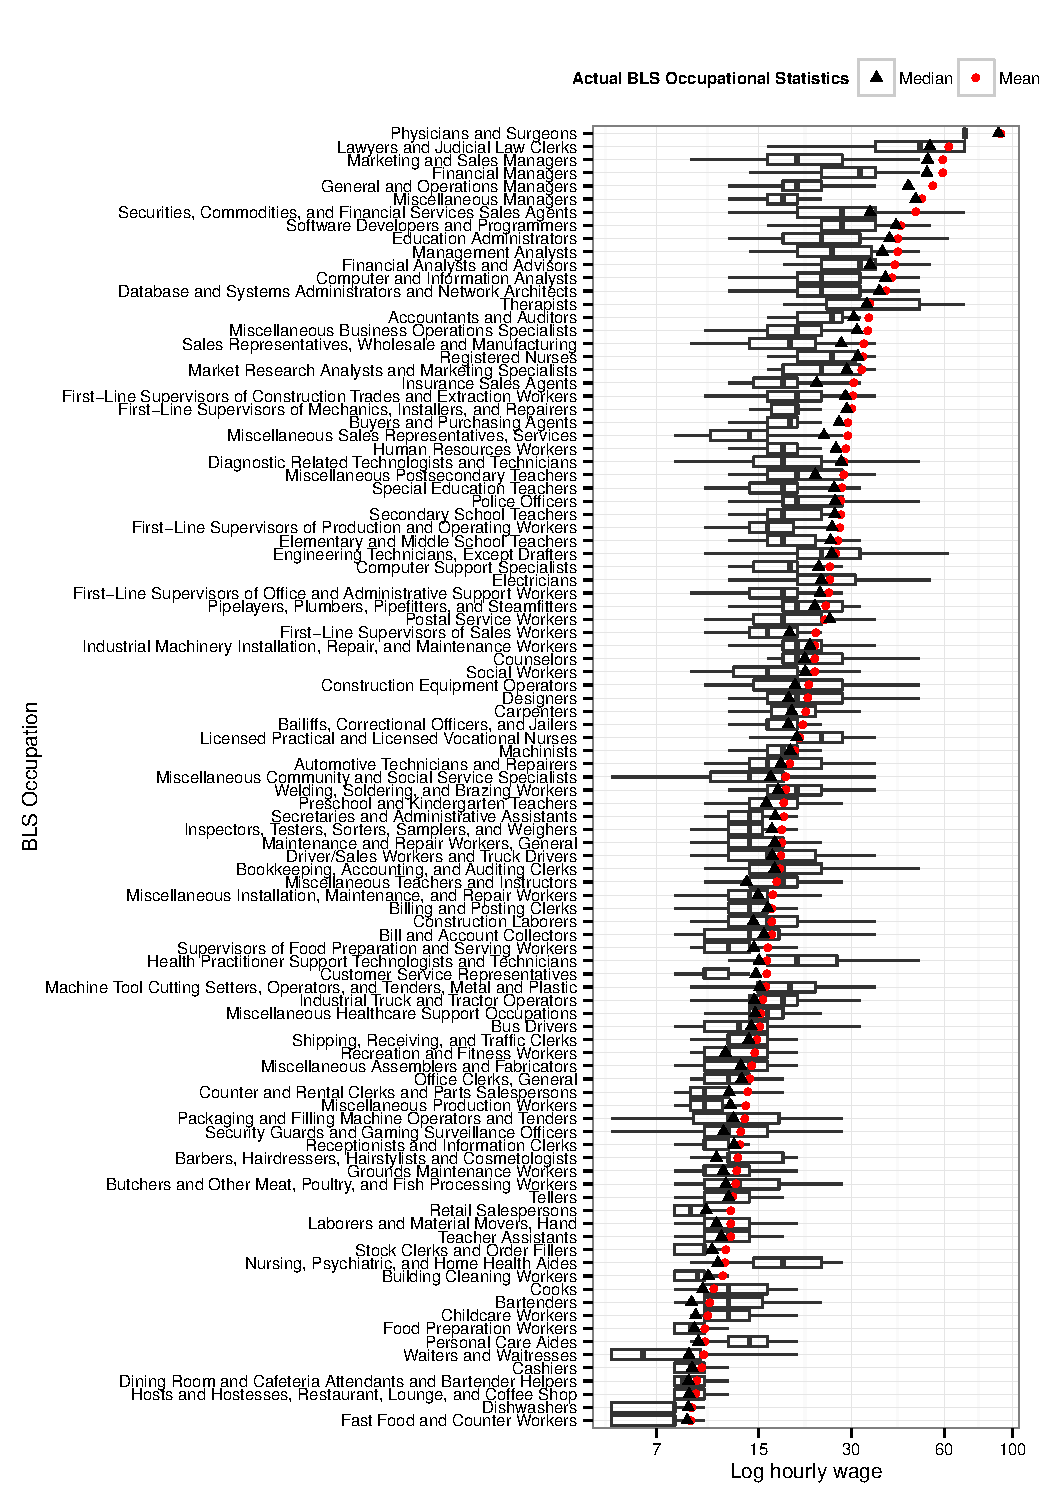
\includegraphics[width = \linewidth]{./plots/box_plots_by_occupation.pdf} 
\emph{Notes:} Boxplots of the respondent wage predictions are shown for each occupation, with actual mean and median over-layed.
\end{minipage}
\end{figure} 


In Figure~\ref{fig:knowledge_by_occupation}, we plot the mean knowledge index by occupations.  

\begin{figure}
\caption{General Knowledge Index by BLS occupation title \label{fig:knowledge_by_occupation}} 
\centering
\begin{minipage}{0.85 \linewidth}
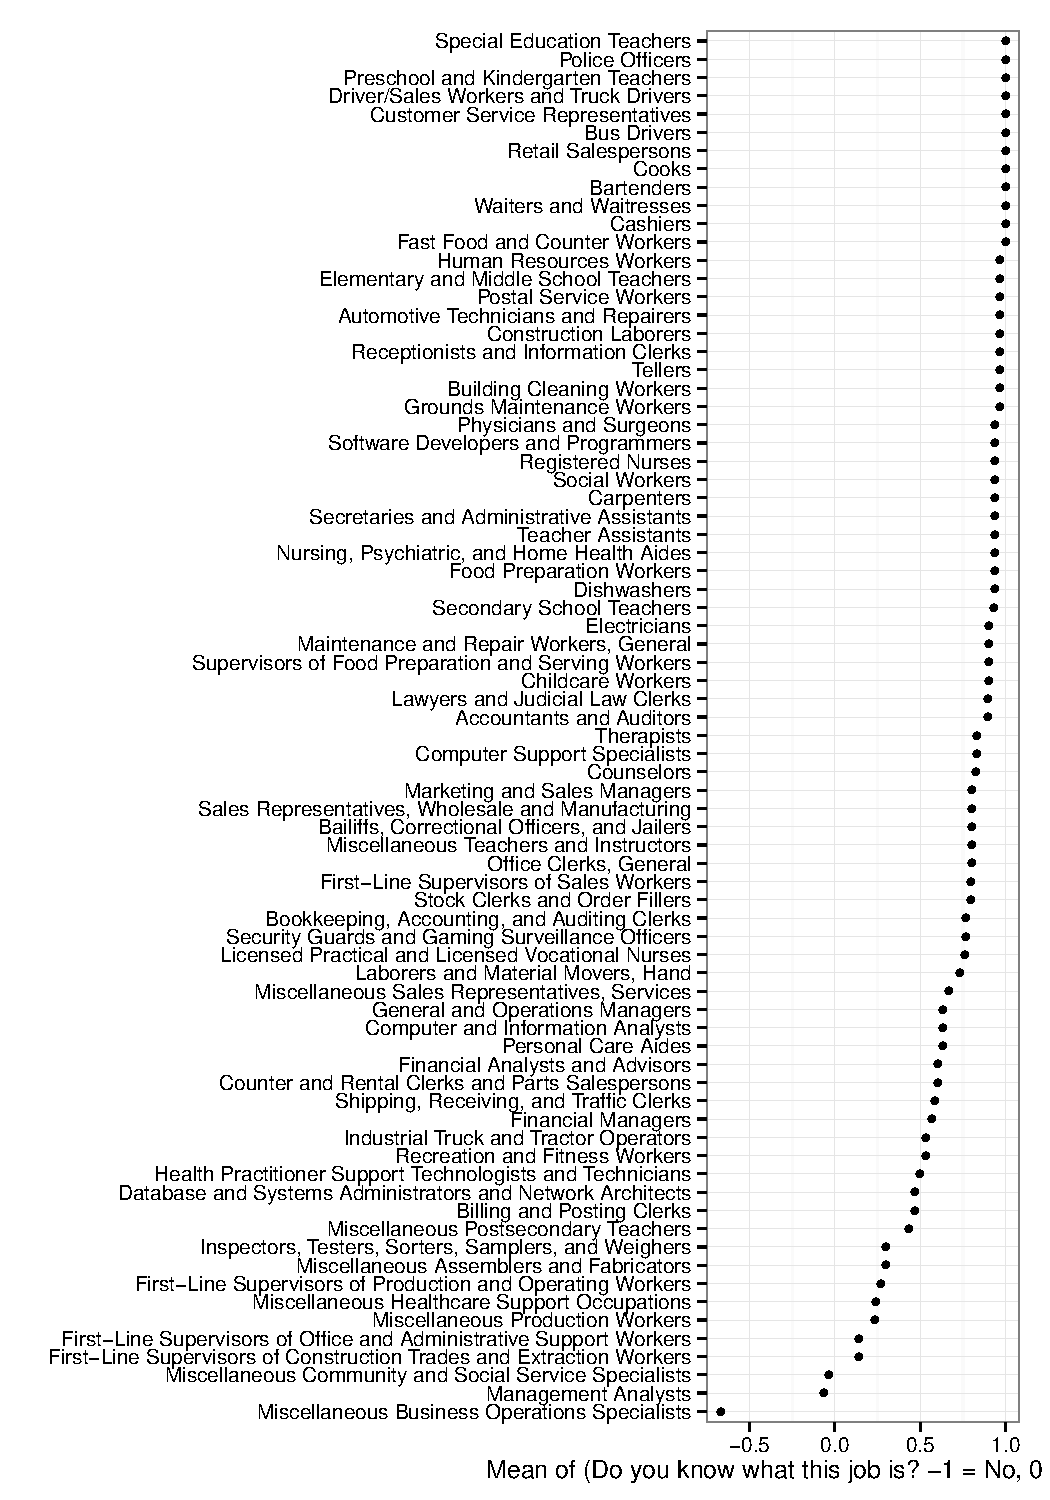
\includegraphics[width = \linewidth]{./plots/knowledge_by_occupation.pdf}
\end{minipage}  
\end{figure} 
%Can we do 0/1 instead of -1/1 so the proportion can be read from the illustration? (proportions are more visceral than these numbers)

\begin{figure}
\caption{Social Knowledge Index by BLS occupation title} \label{fig:social_by_occupation}  
\centering
\begin{minipage}{0.85 \linewidth}
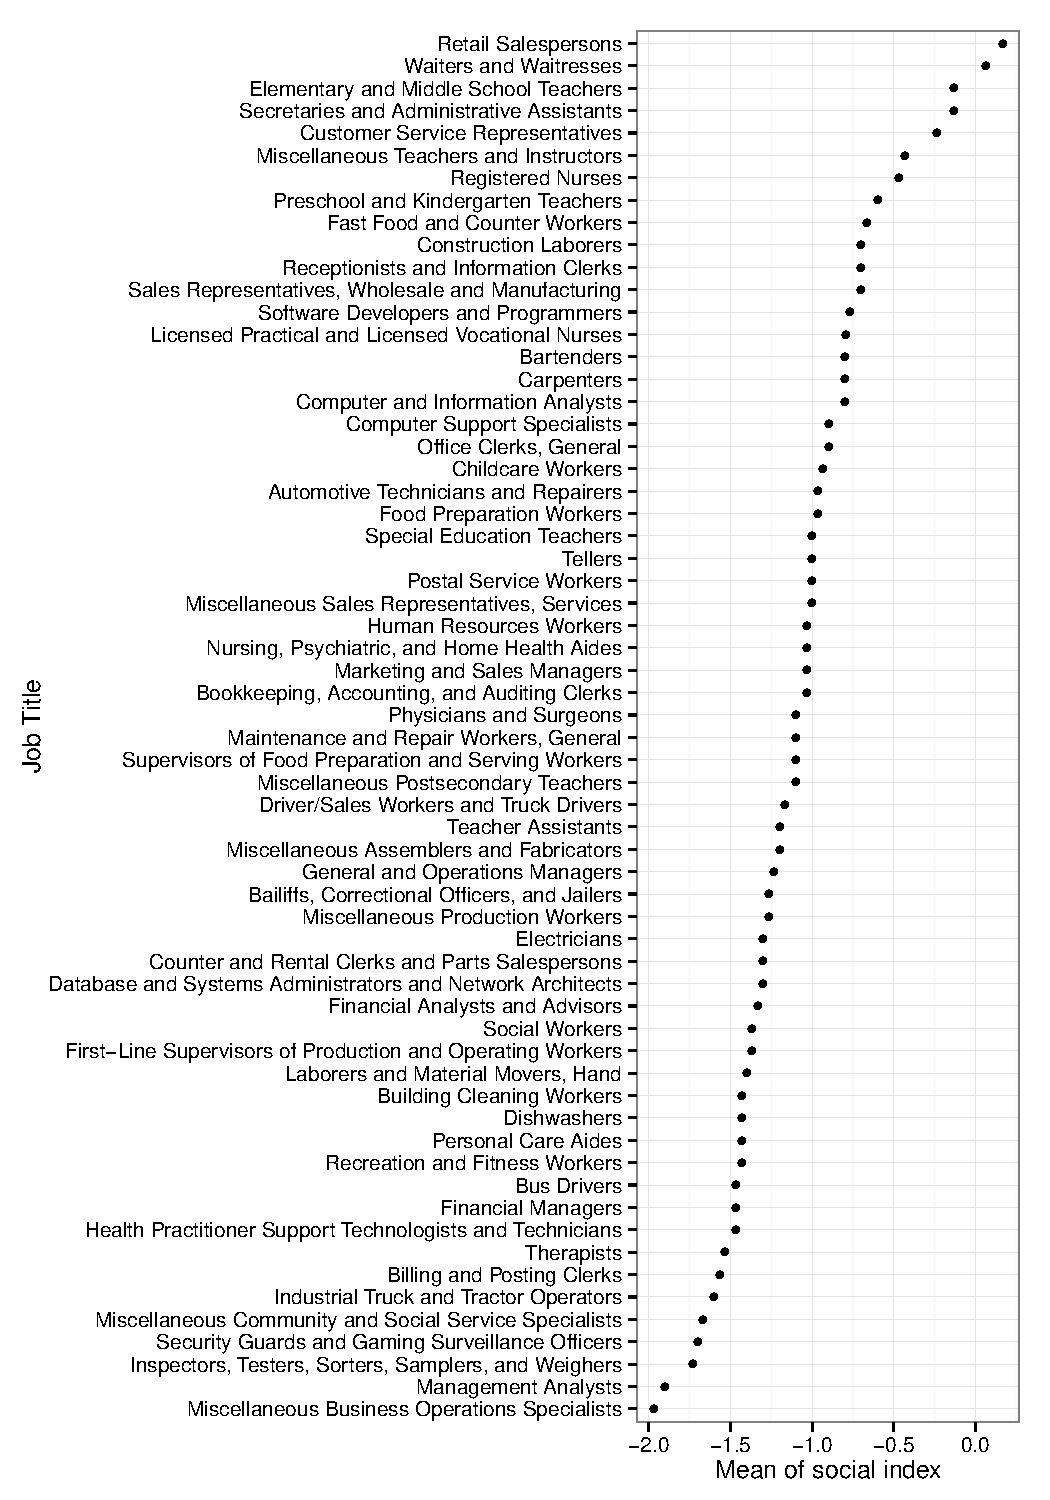
\includegraphics[width = \linewidth]{./plots/social_by_occupation.pdf}
\end{minipage}  
\end{figure} 

% [1] "OCC_CODE"       "OCC_TITLE"      "OCC_GROUP"      "TOT_EMP"       
 [5] "EMP_PRSE"       "H_MEAN"         "A_MEAN"         "MEAN_PRSE"     
 [9] "H_PCT10"        "H_PCT25"        "H_MEDIAN"       "H_PCT75"       
[13] "H_PCT90"        "A_PCT10"        "A_PCT25"        "A_MEDIAN"      
[17] "A_PCT75"        "A_PCT90"        "ANNUAL"         "HOURLY"        
[21] "imputed.hourly"
 [1] "title"               "know.job"            "social.knowledge"   
 [4] "predicted.wage"      "Answer.volume_trend" "Answer.wage_trend"  
 [7] "Answer.comment"      "WorkerId"            "know"               
[10] "social"              "v.trend"             "w.trend"            


\end{document} 
